\newpage 

\subsection{Results and Experiments}

\subsubsection{Final Results}

The described implemented architecture of VAE and VQ-VAE models results show that the models are learning but they are not able to create images that could be interpreted as real.

\begin{figure}[ht]
    \centering
    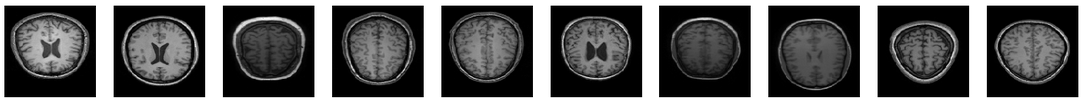
\includegraphics[width = 17cm]{images/mri-real-images.png}
    \caption[Real MR Images]{Real MR Images}
    \label{fig:mri-real-images}
\end{figure}

\begin{figure}[ht]
    \centering
    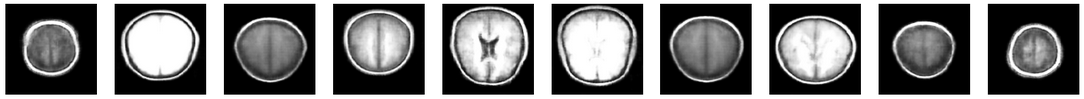
\includegraphics[width = 17cm]{images/vae-brains-results.png}
    \caption[VAE Reconstructed Images]{VAE Reconstructed Images}
    \label{fig:vae-brains-results}
\end{figure}

\begin{figure}[ht]
    \centering
    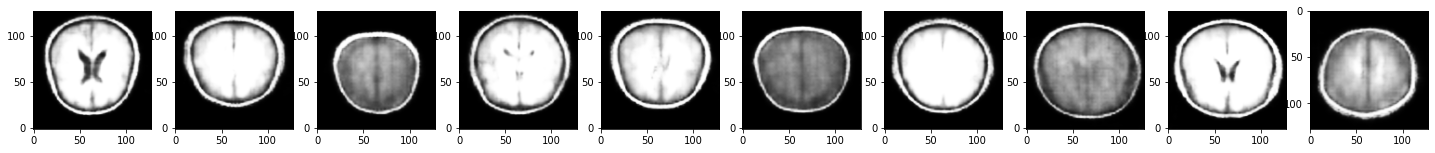
\includegraphics[width = 17cm]{images/vqvae-brains-results.png}
    \caption[VQ-VAE Reconstructed Images]{VQ-VAE Reconstructed Images}
    \label{fig:vqvae-brains-results}
\end{figure}

Reconstructed images are slices that were created using the test data. They were created using the output of the encoder as the decoder input not artificially generated.

Note that real images shown in Figure \ref{fig:mri-real-images} do correlate with images shown in Figures \ref{fig:vae-brains-results} and \ref{fig:vqvae-brains-results}.

\begin{figure}[ht]
    \centering
    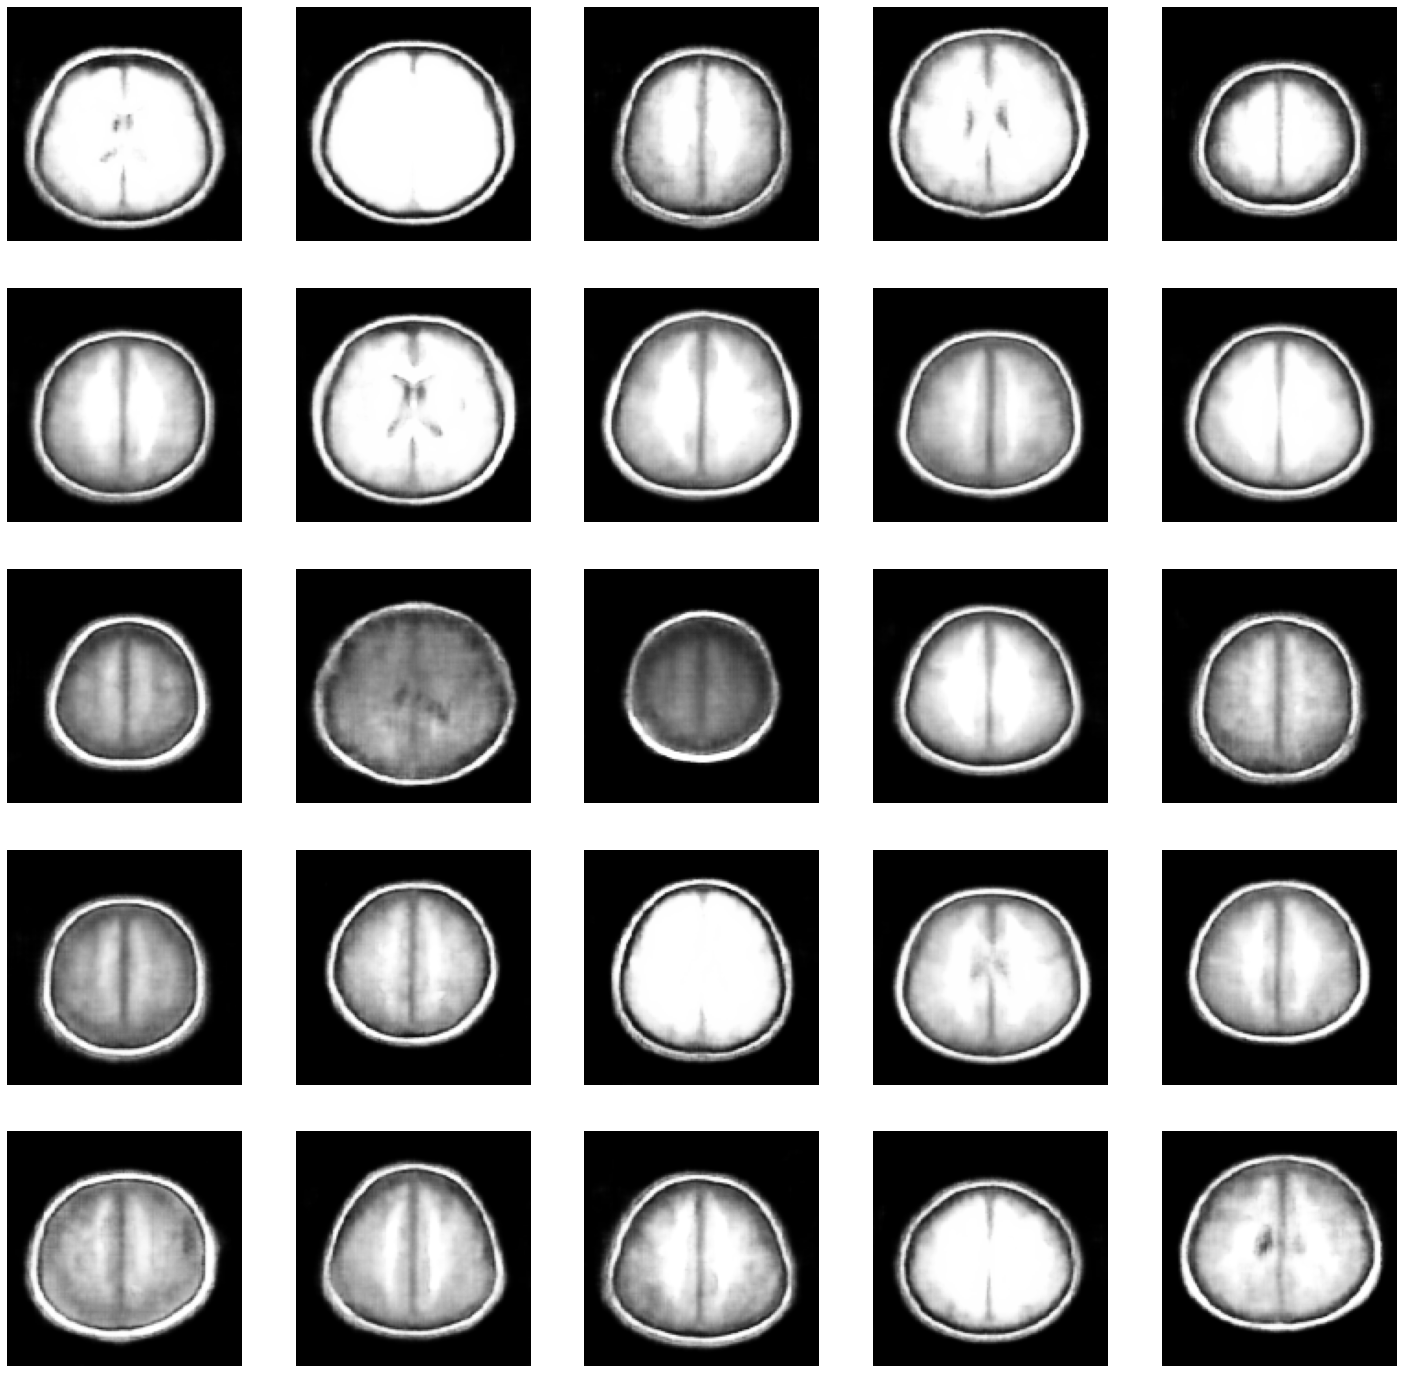
\includegraphics[width = 17cm]{images/vae-brains-results-from-latent-space.png}
    \caption[Artificial VAE images created from latent space]{Artificial VAE images created from latent space}
    \label{fig:vae-images-from-latent-space}
\end{figure}

Looking at technical results, the models seem to learn very slowly but they keep learning even at 500 epochs so the models' limits are yet to be discovered. On the other hand, as explained in dedicated section, VAE model shows an issue with the KL Divergence, it becomes higher over epochs while it must be decreased.

\begin{figure}[ht]
    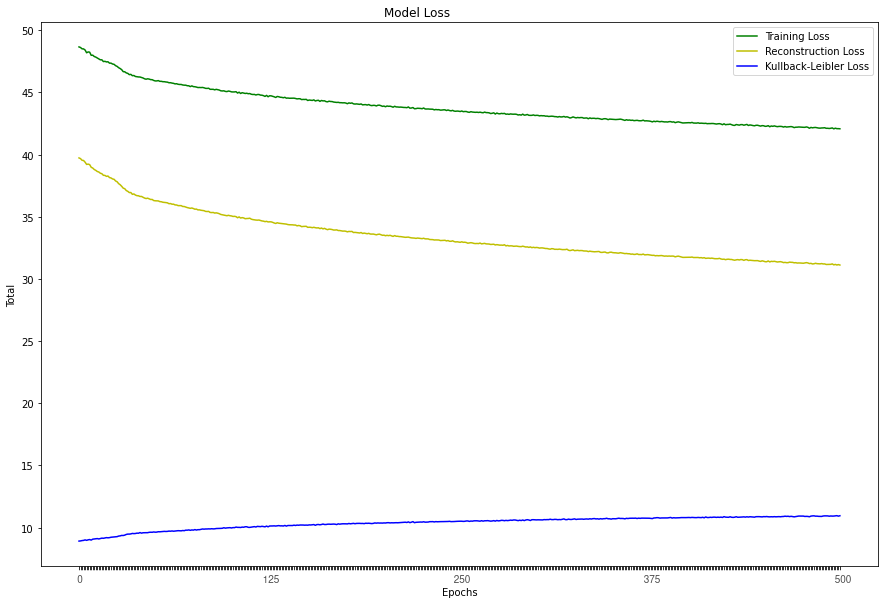
\includegraphics[width = 17cm]{images/vae-loss-results.png}
    \caption[VAE Training loss]{VAE Training loss}
    \label{fig:vae-training-loss}
\end{figure}

\begin{figure}[ht]
    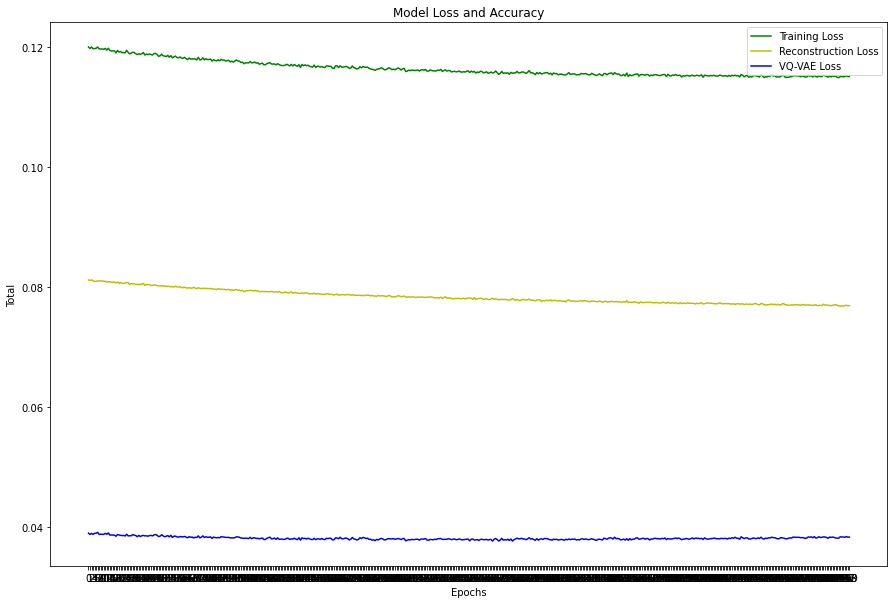
\includegraphics[width = 17cm]{images/vqvae-loss-results.png}
    \caption[VQ-VAE Training loss]{VQ-VAE Training loss}
    \label{fig:vqvae-training-loss}
\end{figure}


% Make sure floats (figures) are placed before new section
\FloatBarrier

\subsubsection{Experiments}

The project implementation methodology followed determined that after every task a fast status analysis was assessed. The reason to do so was the research nature of the project that required continuous evalution on the process and results.

Most of the experiments were executed during the creation of images phase. Whereas the resulting pre-process tasks were overall clear due to  \acrshort{mri} slices deep study, executed at the analysis phase of the project, the creation of images required analysis and implementation cycles since at the analysis phase of the project VAEs' theory was checked but the implementation tasks were not.

Instead of creating it from scratch, a simple \acrfull{cnn} that is used to show VAE example on MNIST \cite{mnist} digits was picked. It was only used to test the code functionality only, results were not important and they were discarded. 

Once that the functionality was proved to work, the 5-block network was implemented with the following features (details only the ones that vary from the final model):

\begin{itemize}
    \item 128, 64, 32, 16 and 8 dimensions and a latent space of 200
    \item kernel size was 3
    \item trained on 30 epochs only
    \item 256 pixels
\end{itemize}

Producing the images shown in Figure \ref*{fig:vae-k3-brains-30-epochs} and losses shown in Figure \ref*{fig:vae-k3-loss-30-epochs}

\begin{figure}[ht]
    \centering
    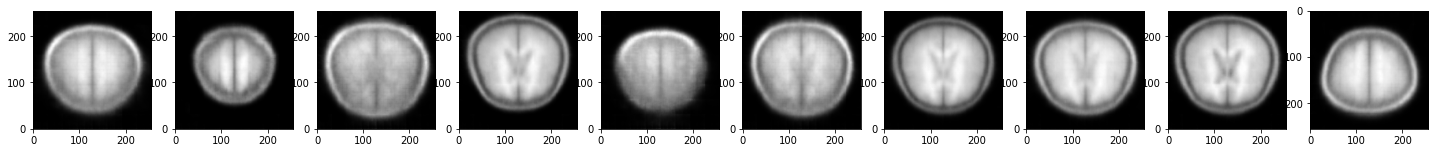
\includegraphics[width = 17cm]{images/vae-k3-brains-30-epochs.png}
    \caption[VAE Results on experiments I]{VAE Results on experiments I}
    \label{fig:vae-k3-brains-30-epochs}
\end{figure}

\begin{figure}[ht]
    \centering
    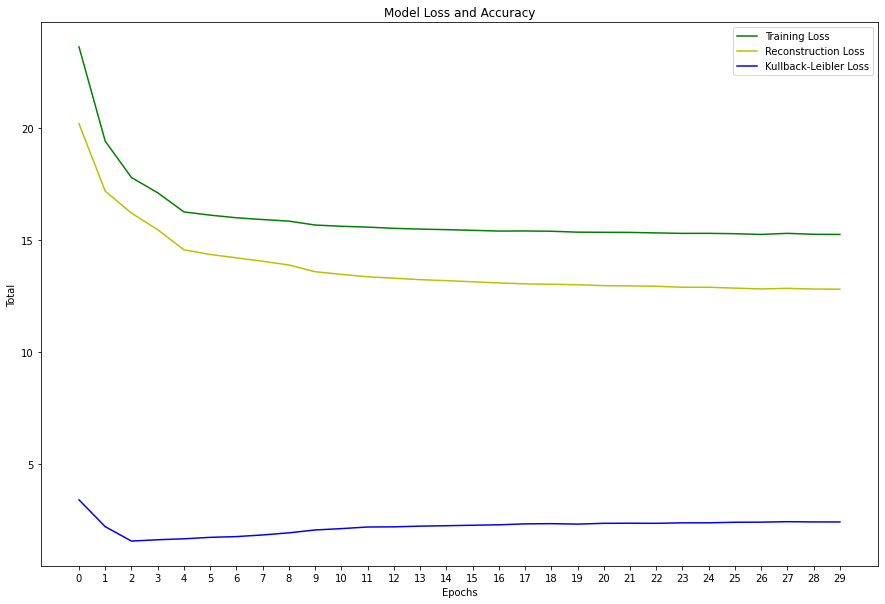
\includegraphics[width = 14cm, height=8cm]{images/vae-k3-loss-30-epochs.png}
    \caption[VAE Losses on experiments I]{VAE Losses on experiments I}
    \label{fig:vae-k3-loss-30-epochs}
\end{figure}

At that time, since results on images were not ideal the new approach was created in order to double-check if the kl-divergence issue could be the reason for not getting better results. A VQ-VAE implementation was created along with an extra sixth layer added at the begining of the encoder, looking for a slower learning approach. The VQ-VAE implementation with 6 layers produced the images shown in Figure \ref*{fig:vqvae-6layers-30-epochs} and losses shown in Figure \ref*{fig:vqvae-6layers-loss-30-epochs}

\begin{figure}[ht]
    \centering
    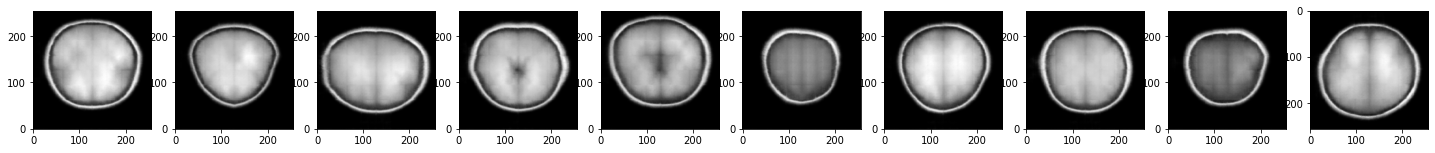
\includegraphics[width = 17cm]{images/vqvae-6layers-30-epochs.png}
    \caption[VQ-VAE Results on experiments II]{VQ-VAE Results on experiments II}
    \label{fig:vqvae-6layers-30-epochs}
\end{figure}

\begin{figure}[ht]
    \centering
    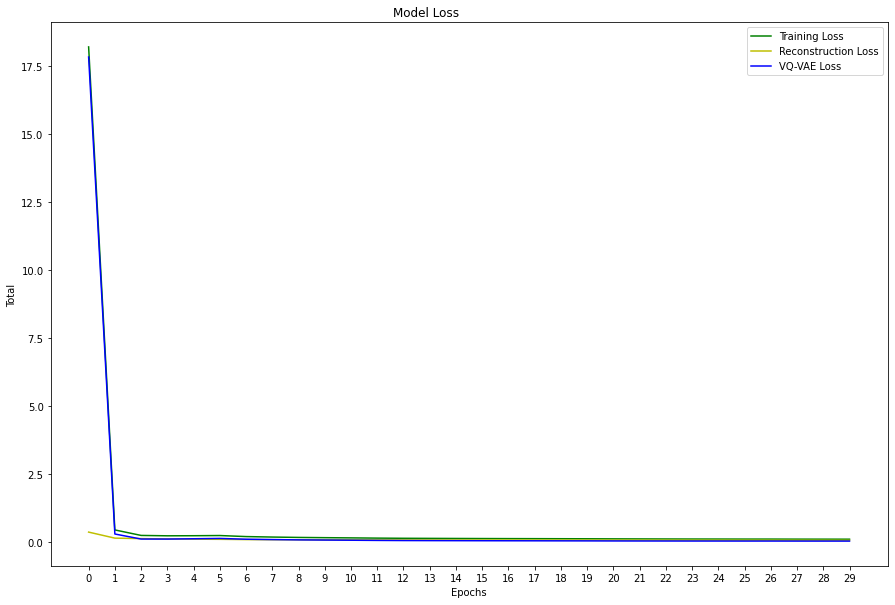
\includegraphics[width = 14cm, height=8cm]{images/vqvae-6layers-loss-30-epochs.png}
    \caption[VQ-VAE Losses on experiments II]{VQ-VAE Losses on experiments II}
    \label{fig:vqvae-6layers-loss-30-epochs}
\end{figure}

Then, after checking that VAE and VQ-VAE produced similar results it was decided to look into different angles of potential improvements and the downsampling of pixels experiment was chosen to be next. Along with downsampling, the number of epochs was increased to 200.

VAE Produced the images shown in Figure \ref*{fig:vae-brains-128pixels-200epochs} and losses shown in Figure \ref*{fig:vae-loss-128pixels-200epochs}

\begin{figure}[ht]
    \centering
    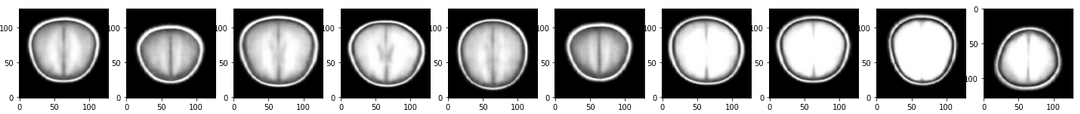
\includegraphics[width = 17cm]{images/vae-brains-128pixels-200epochs.png}
    \caption[VAE Results on experiments III]{VAE Results on experiments III}
    \label{fig:vae-brains-128pixels-200epochs}
\end{figure}

\begin{figure}[ht]
    \centering
    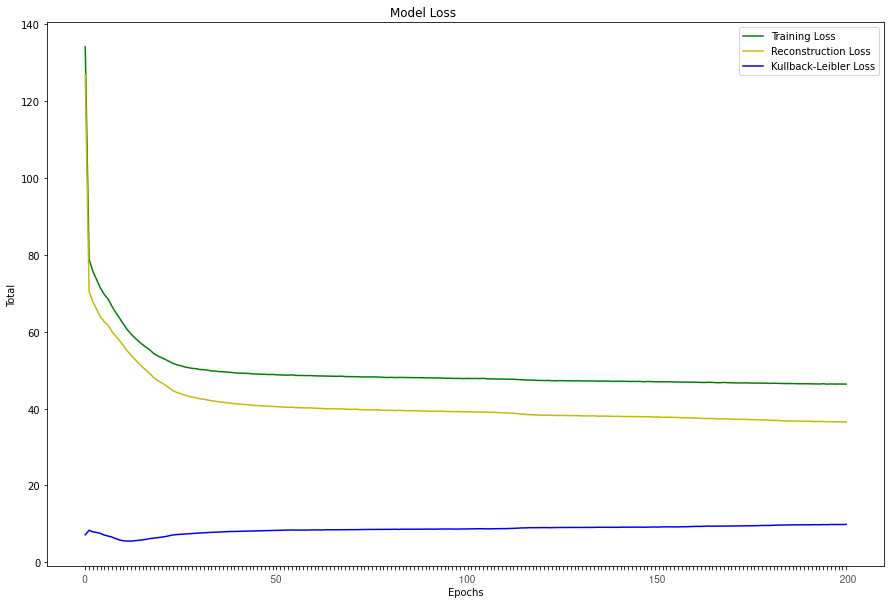
\includegraphics[width = 14cm, height=8cm]{images/vae-loss-128pixels-200epochs}
    \caption[VAE Losses on experiments III]{VAE Losses on experiments III}
    \label{fig:vae-loss-128pixels-200epochs}
\end{figure}

After that, some other parameters changes were tested with no remmarkable results compared to the latest results obtained. Tested parameters were learning rates 0.0001, 0.0005 and kernel size 3, trained on 500 epochs.